\chapter{Analisis}
\section{Analisis Sistem}
Analisis sistem dapat didefinisikan sebagai penguraian dari suatu sistem informasi yang utuh kedalam bagian-bagian komponennya dengan maksud untuk mengidentifikasi dan mengevaluasi urutan algoritma dan fungsi-fungsi dalam sistem yang berjalan. Pada bagian ini, akan dibahas mengenai Analisis Aplikasi Downloader Mp4 Youtube akan digambarkan dalam bentuk \textit{flowmap} dan \textit{data flow diagram}.

\subsection{Analisis Sistem yang sedang berjalan}
Untuk gambaran sistem yang berjalan dalam aplikasi Downloader Mp4 Youtube adalah proses dimana informasi yang terdapat pada aplikasi dapat digunakan sebagai media mendownload video yang terdapat pada aplikasi Downloader Mp4 Youtube. 

\subsubsection{Analisis Prosedur (Flowmap)}
Prosedurnya di awali dari user membuka aplikasi website Downloader Mp4 Youtube {(savefrom.net)}kemudian membuka Youtube sebagai media penyedia video .

\begin{enumerate}
    \item Mulai.
    \item Mambuka website Youtube lalu cari video yang di inginkan kemudian copy URL video Youtube tersebut.
    \item Pada tab lain buka website aplikasi Downloader Mp4 Youtube {(savefrom.net)}.
    \item Kemudian tempel url video Youtube pada aplikasi Downloader Mp4 Youtube {(savefrom.net)}.
    \item kemudian anda dapat memilih kulitas unduhan seperti Mp4 serta WEBM.
    \item Jika sudah menentukan kualiatas, anda dapat menekan tombol download 
    \item Setelah itu User dapat menerima notifikasi serta tujuan penyimpanan download video atau musik.
    \item Selesai.
\end{enumerate}

\begin{figure}[!htbp]
    \centering
    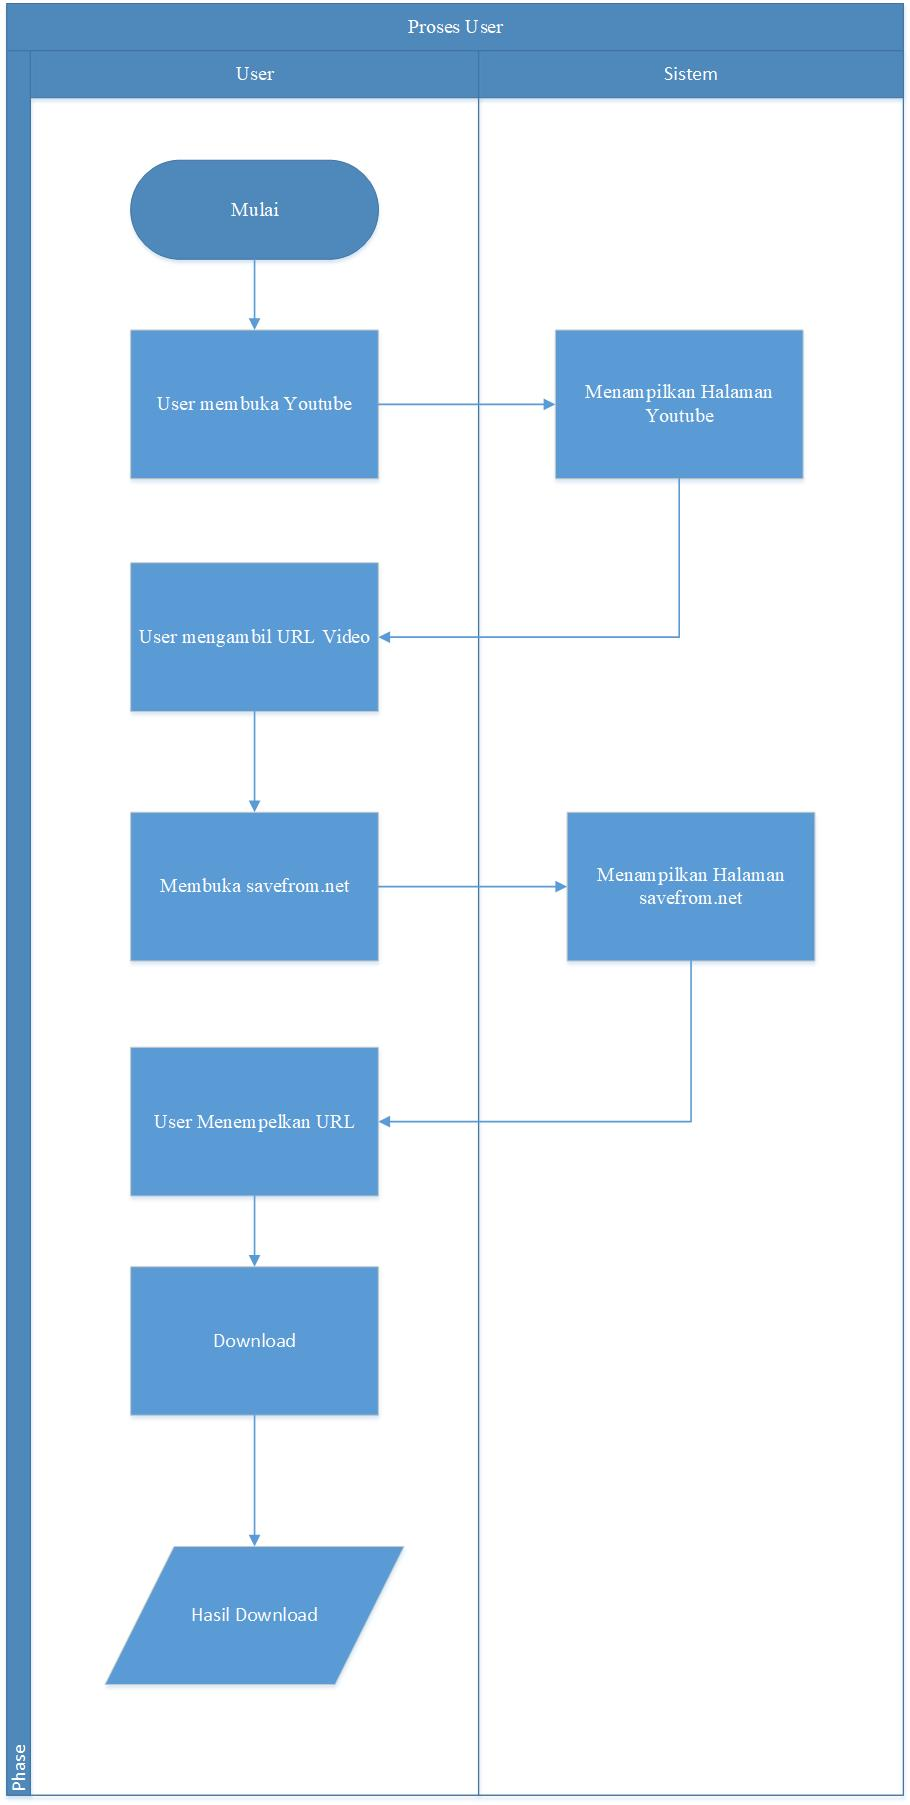
\includegraphics[scale=0.6]{figure/Drawing2.jpg}
    \caption{\textit{flowmap Mp4 youtube yang berjalan }}
    \label{gambar 1}
\end{figure}

\subsection{Kebutuhan Perangkat lunak }
Kebutuhan perangkat lunak dimaksud disini adalah berupa software pendukung yang bisa digunakan pada proses berjalannya aplikasi Downloader Mp4 Youtube :
\begin{enumerate}
    \item Anaconda 3 2019.07 64-bit
    \item Spyder 3.3.6 64-bit
    \item Python 3.7.3 64-bit
    \item firefox quantum 69.0.1 64-bit
\end{enumerate}

\section{Analisis DFD}
\subsection{Data Flow Diagram}
Data Flow Diagram adalah salah satu cara untuk menjelaskan sistem secara logika bagaimana arus data yang berjalan dalam sistem tersebut.

\subsubsection{Data Flow Diagram Level 0}
Data Flow Diagram level 0 merupakan penjelasan dasar arus informasi dari Youtube dan aplikasi Downloader Mp4 {(savefrom.net)}.

\begin{figure}[!htbp]
    \centering
    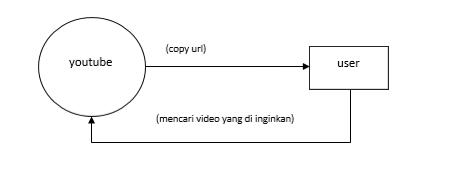
\includegraphics[scale=1]{figure/youtube.jpeg}
    \caption{\textit{DFD level 0 dari youtube}}
    \label{gambar 1}
\end{figure}


Data Flow Diagram level 0 pada youtube, mencakup:
\begin{enumerate}
    \item Berisi 2 Entitas, yaitu user dan admin.
    \item Kemudian berisi 1 Proses, dari Youtube.
\end{enumerate}

\begin{figure}[!htbp]
    \centering
    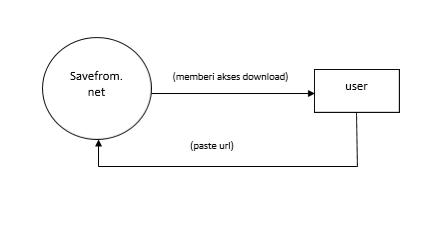
\includegraphics[scale=1]{figure/savefrom.jpeg}
    \caption{\textit{DFD level 0 dari savefrom.net}}
    \label{gambar 1}
\end{figure}
\vspace{1cm}
Data Flow Diagram level 0 pada aplikasi savefrom.net, mencakup:
\begin{enumerate}
    \item Berisi 2 Entitas, yaitu user dan admin.
    \item Kemudian berisi 1 Proses, yaitu aplikasi Downloader Mp4 Youtube.
\end{enumerate}

\vspace{8cm}

\subsection{Spesifikasi Tabel}
\subsubsection{Spesifikasi Proses DFD Level 0}

Berikut spesifikasi proses DFD level 0 pada youtube dan savefrom.net terdapat  pada tabel \ref{tableSpec1}

\begin{table}[!htbp]
\centering
\caption{Tabel Spesifikasi}
\label{tableSpec1}
\begin{tabular}{|l|l|l|l|l|}
\hline
No & Proses & Masukan & Keluaran & Logika Proses \\
\hline

 & & & & \textit{Begin if}\\
 & & & & jika judul di: \\
 & & & & \textit{input} maka muncul  \\
 & & & & video \\
 & & \textit{input} judul& menampilkan \\
1 &  Youtube & video & video & \textit{else if} \\
 & & & dan url& judul = valid \\
 & & & & \textit{then} \\
 & & & & tampilkan video dan url \\
 & & & & \textit{Endif} \\
\hline

 & & & & \textit{Begin if}\\
 & & & & jika url: \\
 & & & & terbaca maka muncul  \\
 & & & & video \\
 & & \textit{copy link} & menampilkan  & hasil dari Youtube \\
1 &  Aplikasi savefrom.net &url& link & \textit{else if} \\
 & & & download& url = valid \\
 & & & & \textit{then} \\
 & & & & tampilkan menu download \\
 & & & & \textit{Endif} \\
\hline

\end{tabular}
\end{table}

\subsection{Testing}
Antar muka atau \textit{User Interface} (UI) adalah cara sebuah program berinteraksi langsung dengan pengguna dengan kata lain segala sesuatu dirancang menjadi sebuah perangkat informasi sehingga pengguna dapat lebih mudah melakukan interaksi dengan program. Dalam merancang sebuah user interface kita harus memperhatikan beberapa hal:
\begin{enumerate}
    \item User Interface yang sederhana, maksudnya didalam aplikasi tersebut tidak ada elemen fungsi yang kira kiranya tidak diperlukan dan hanya terdapat elemen yang dibutuhkan oleh pengguna.
    \item User Interface juga dibentuk sesuai siapa pengguna aplikasi tersebut. Sehingga dapat menyesuaikan kemampuan dan pengalaman user dalam berinteraksi.
    \item Penempatan layout agar tidak memepersulit pengguna dalam menggunakan sebuah aplikasi.
 
\end{enumerate} 
\subsubsection{Perancangan Antar Muka yang Sedang Berjalan}
Antar Muka yang sedang berjalan dalam aplikasi Downloader Mp4 adalah bagaimana alur proses dari pembukaan Youtube sampai download video pada aplikasi savefrom.net.

\begin{figure}[!htbp]
    \centering
    
\includegraphics[scale=1.5]{figure/CMD.png}
    \caption{Proses pada cmd }
    \label{gambar 1}
\end{figure}

\begin{figure}[!htbp]
    \centering
    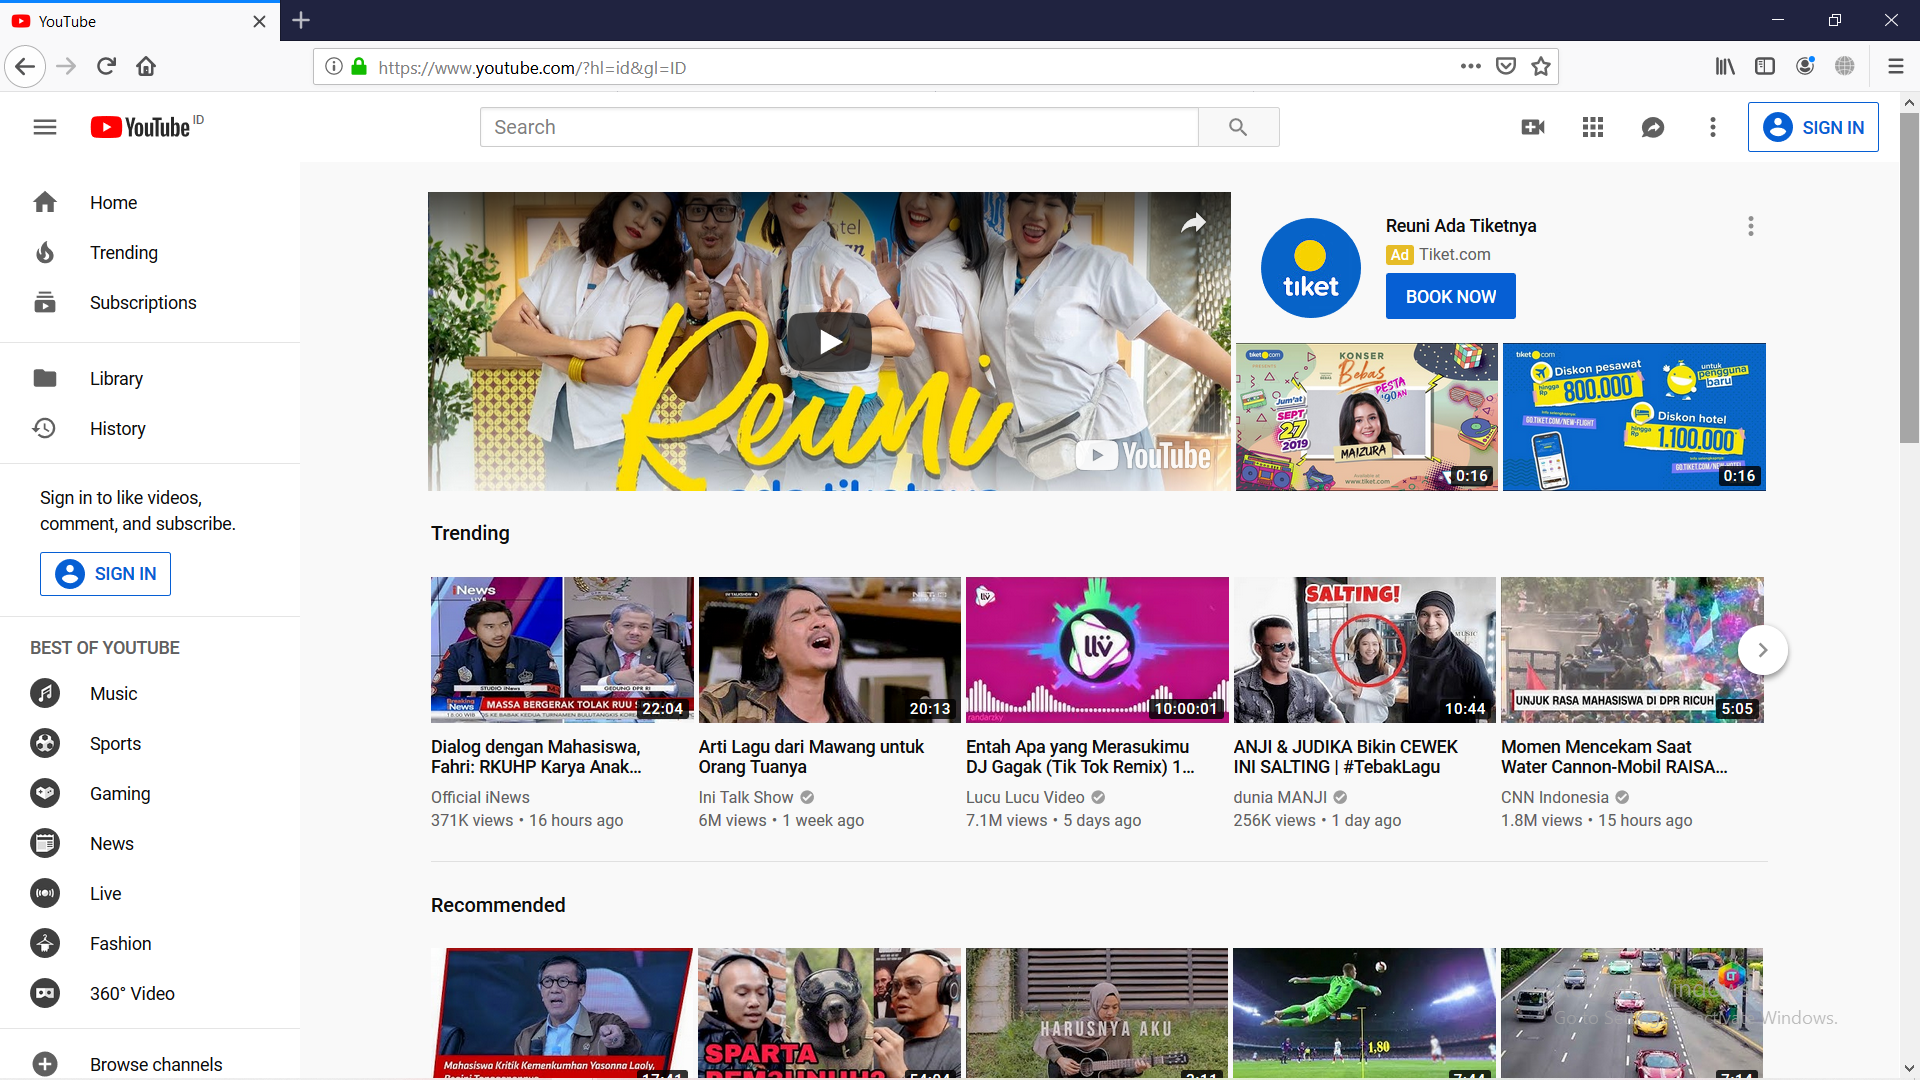
\includegraphics[scale=0.4]{figure/Antarmuka/1.png}
    \caption{ Proses pada Pembukaan youtube}
    \label{gambar 1}
\end{figure}

\begin{figure}[!htbp]
    \centering
    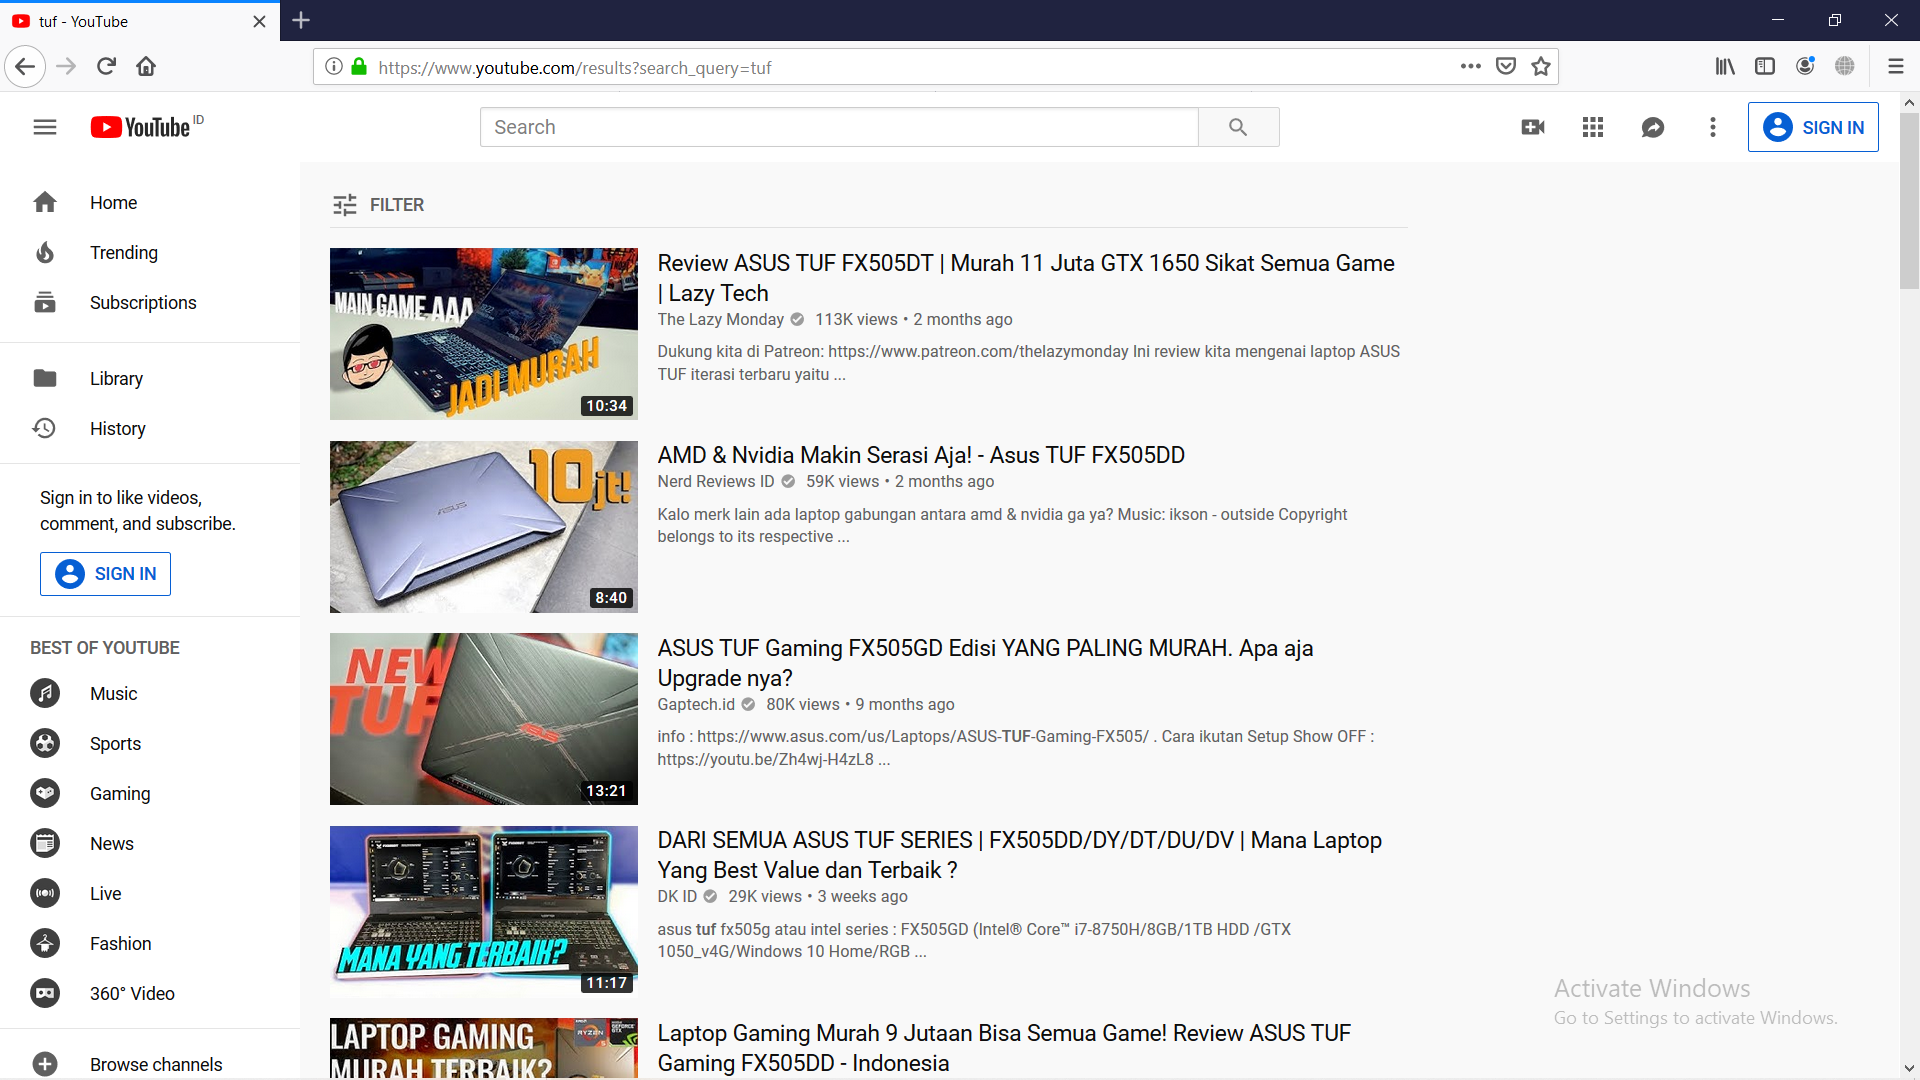
\includegraphics[scale=0.4]{figure/Antarmuka/2.png}
    \caption{ Proses pada saat mencari video}
    \label{gambar 1}
\end{figure}

\begin{figure}[!htbp]
    \centering
    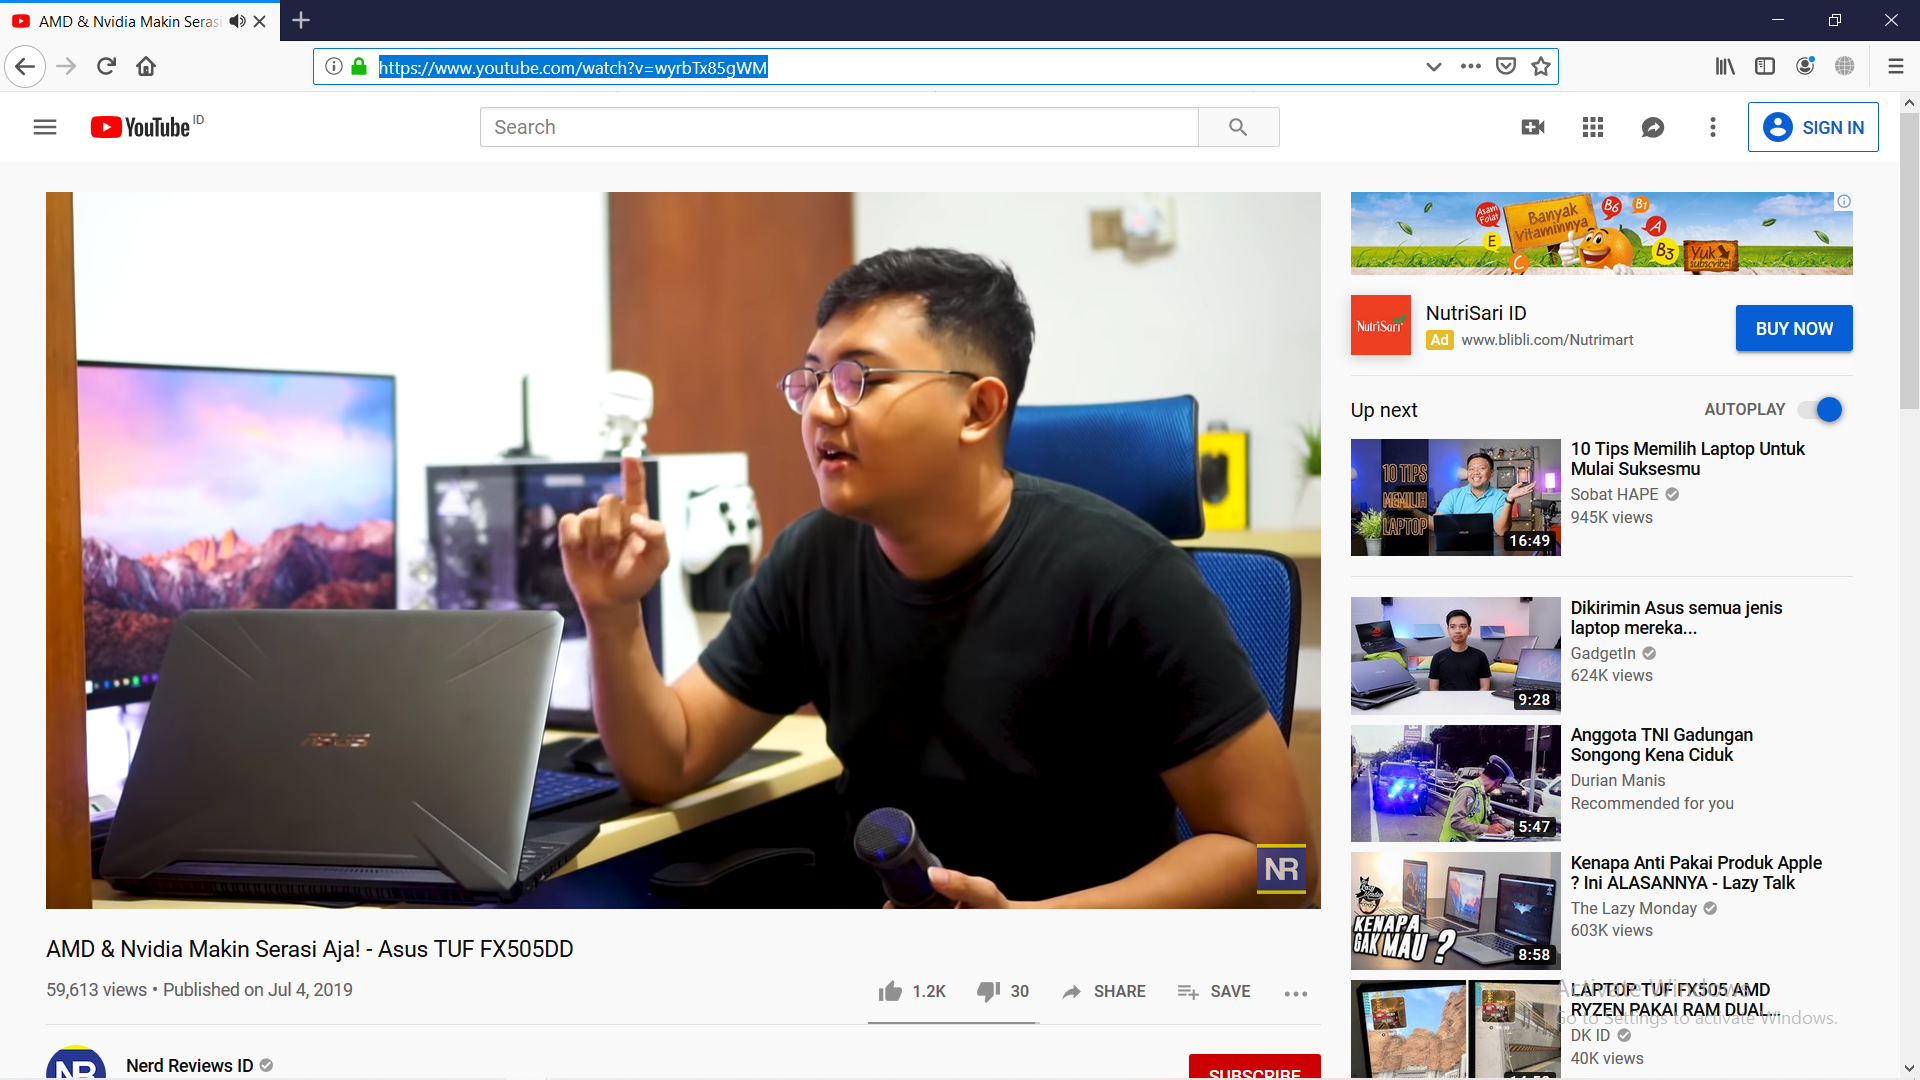
\includegraphics[scale=0.4]{figure/Antarmuka/3.png}
    \caption{ Proses saat mengambil Url video}
    \label{gambar 1}
\end{figure}

\begin{figure}[!htbp]
    \centering
    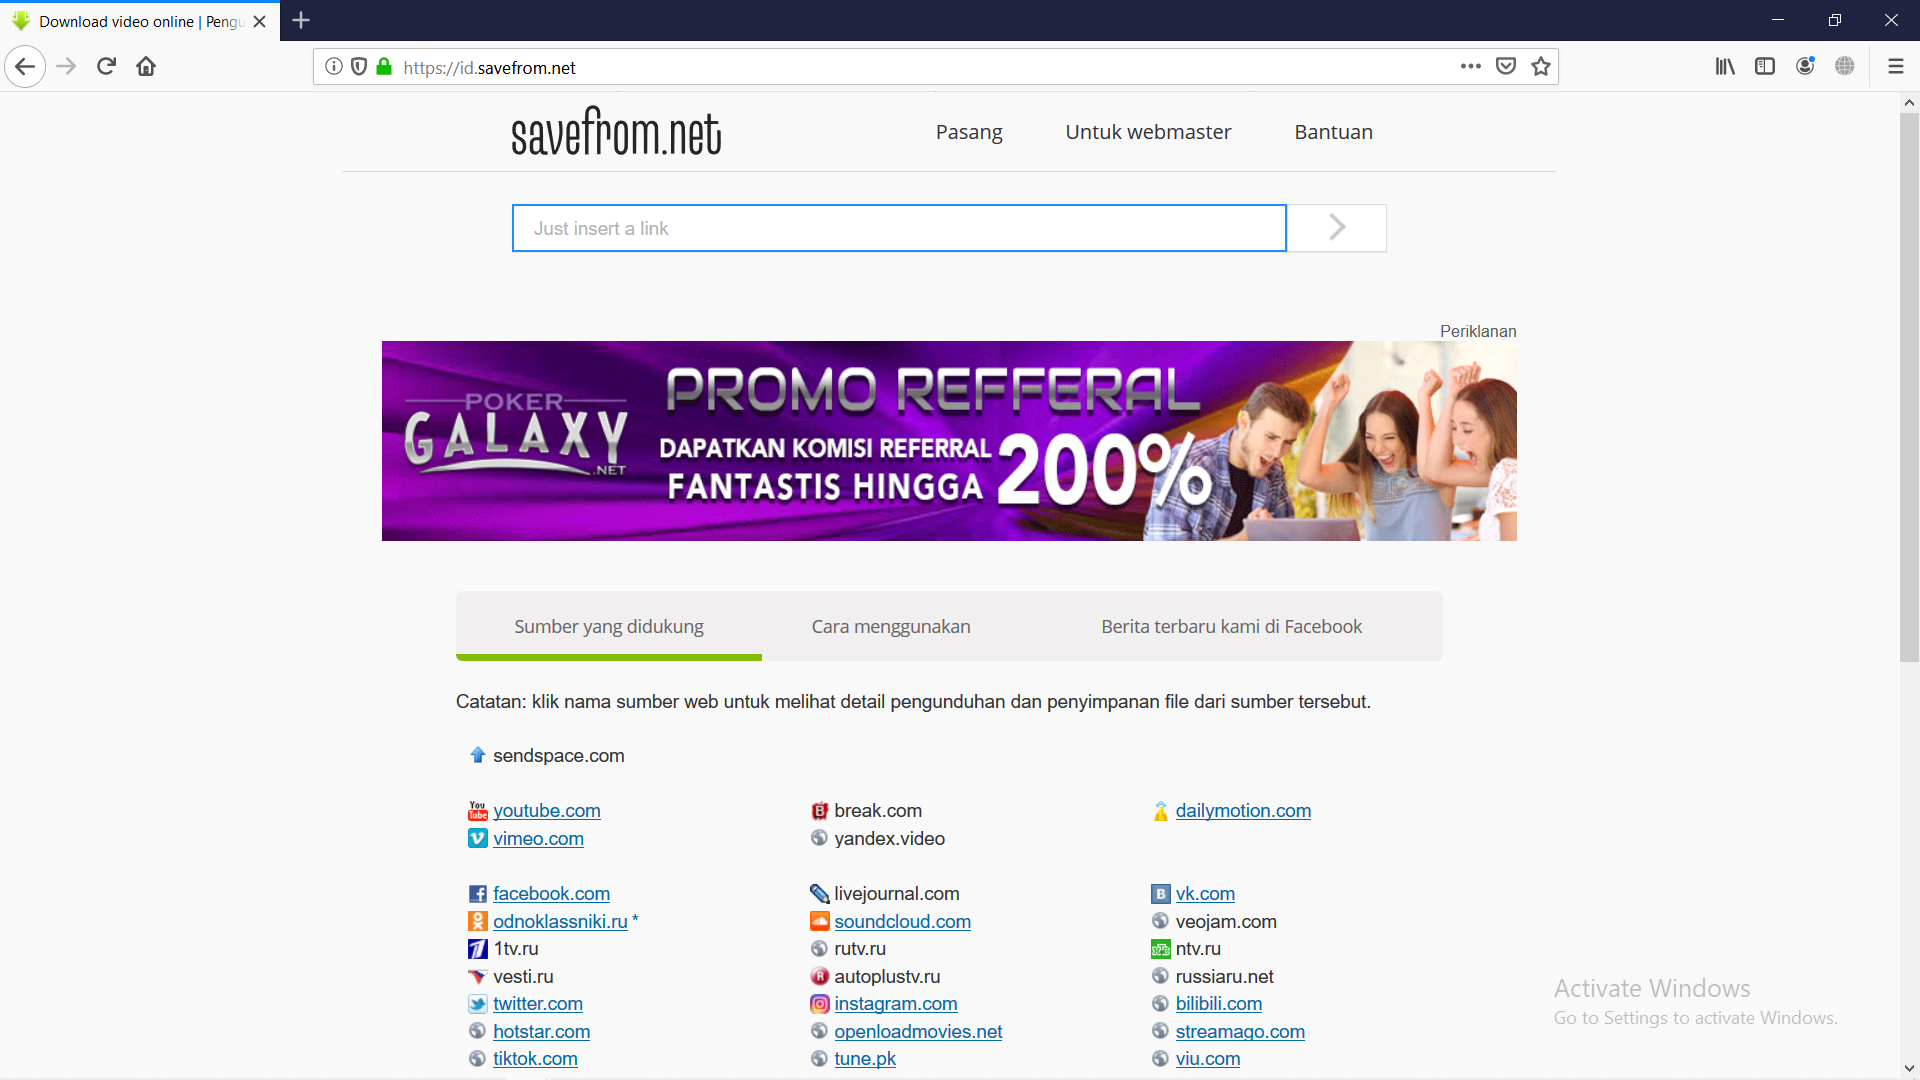
\includegraphics[scale=0.4]{figure/Antarmuka/4.png}
    \caption{ Proses saat membuka savefrom.net}
    \label{gambar 1}
\end{figure}


\begin{figure}[!htbp]
    \centering
    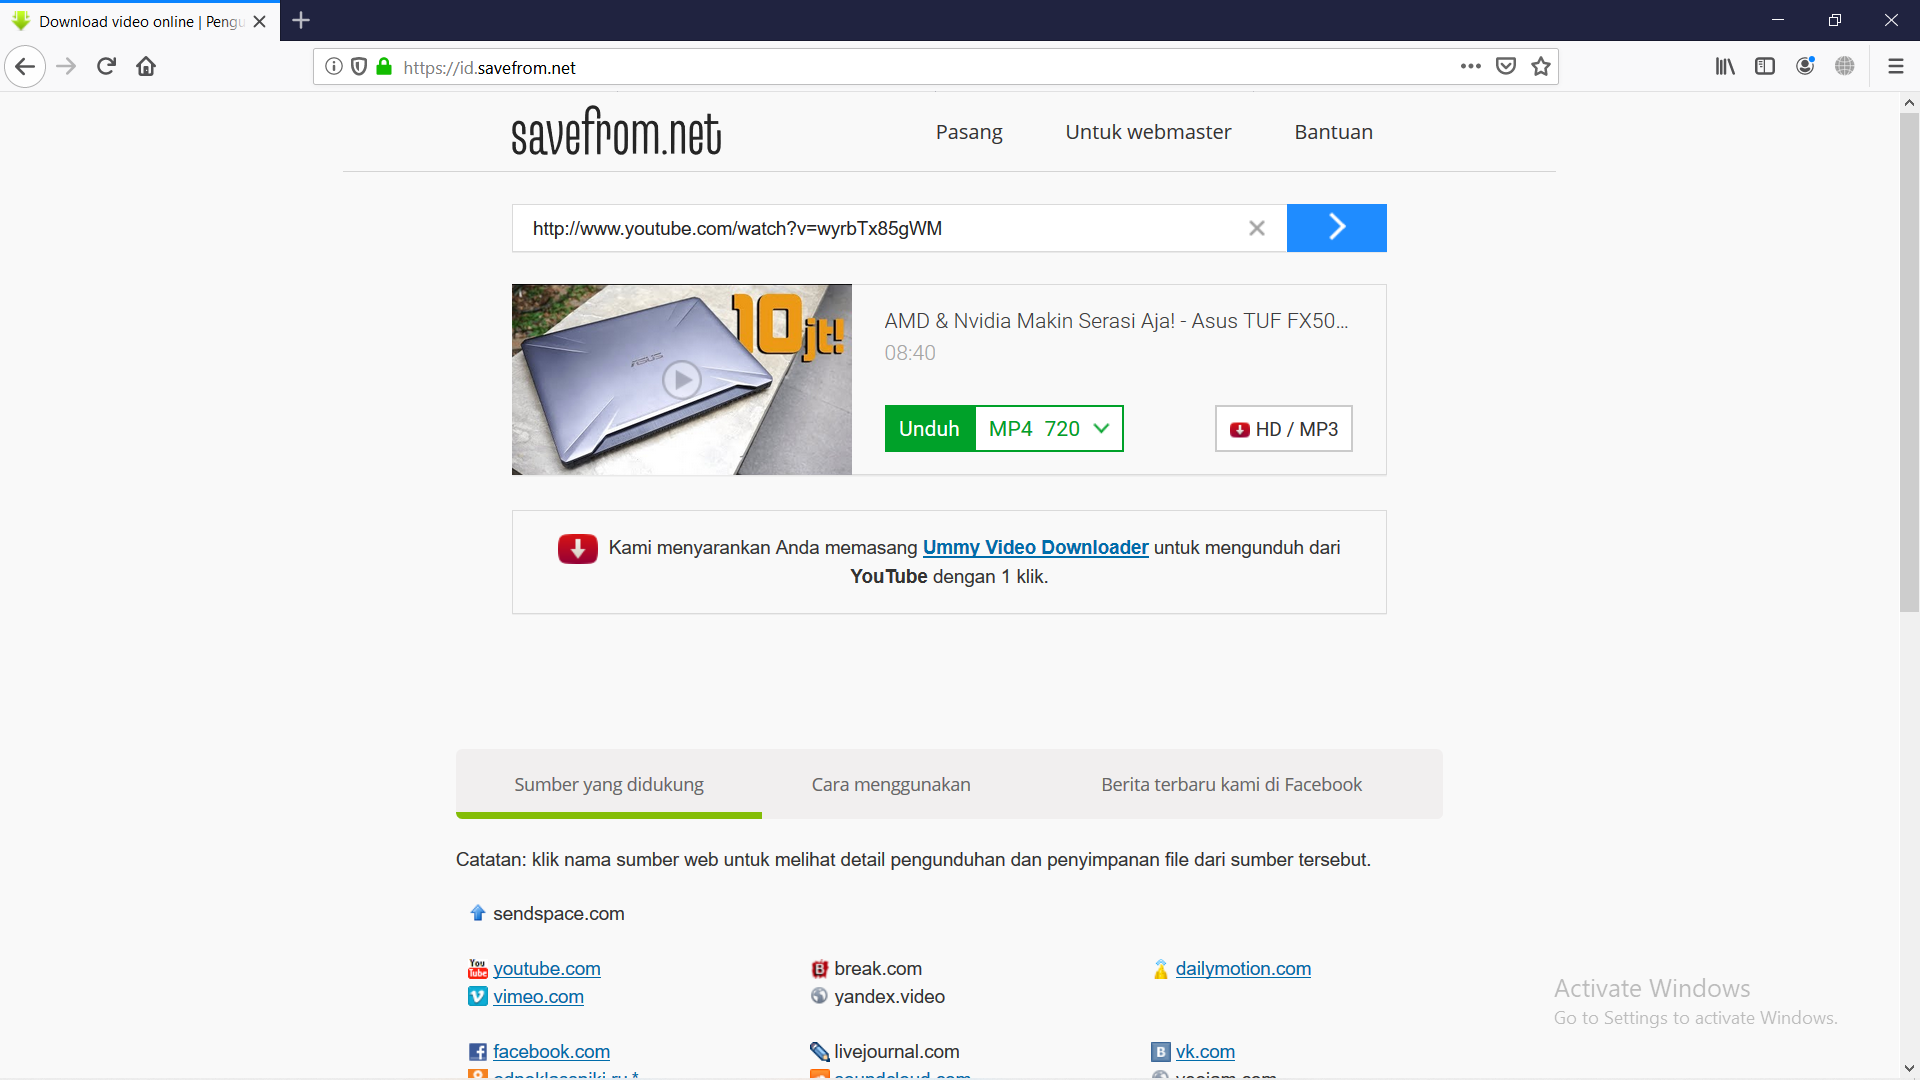
\includegraphics[scale=0.4]{figure/Antarmuka/5.png}
    \caption{Proses saat copy url pada savefrom.net}
    \label{gambar 1}
\end{figure}

\begin{figure}[!htbp]
    \centering
    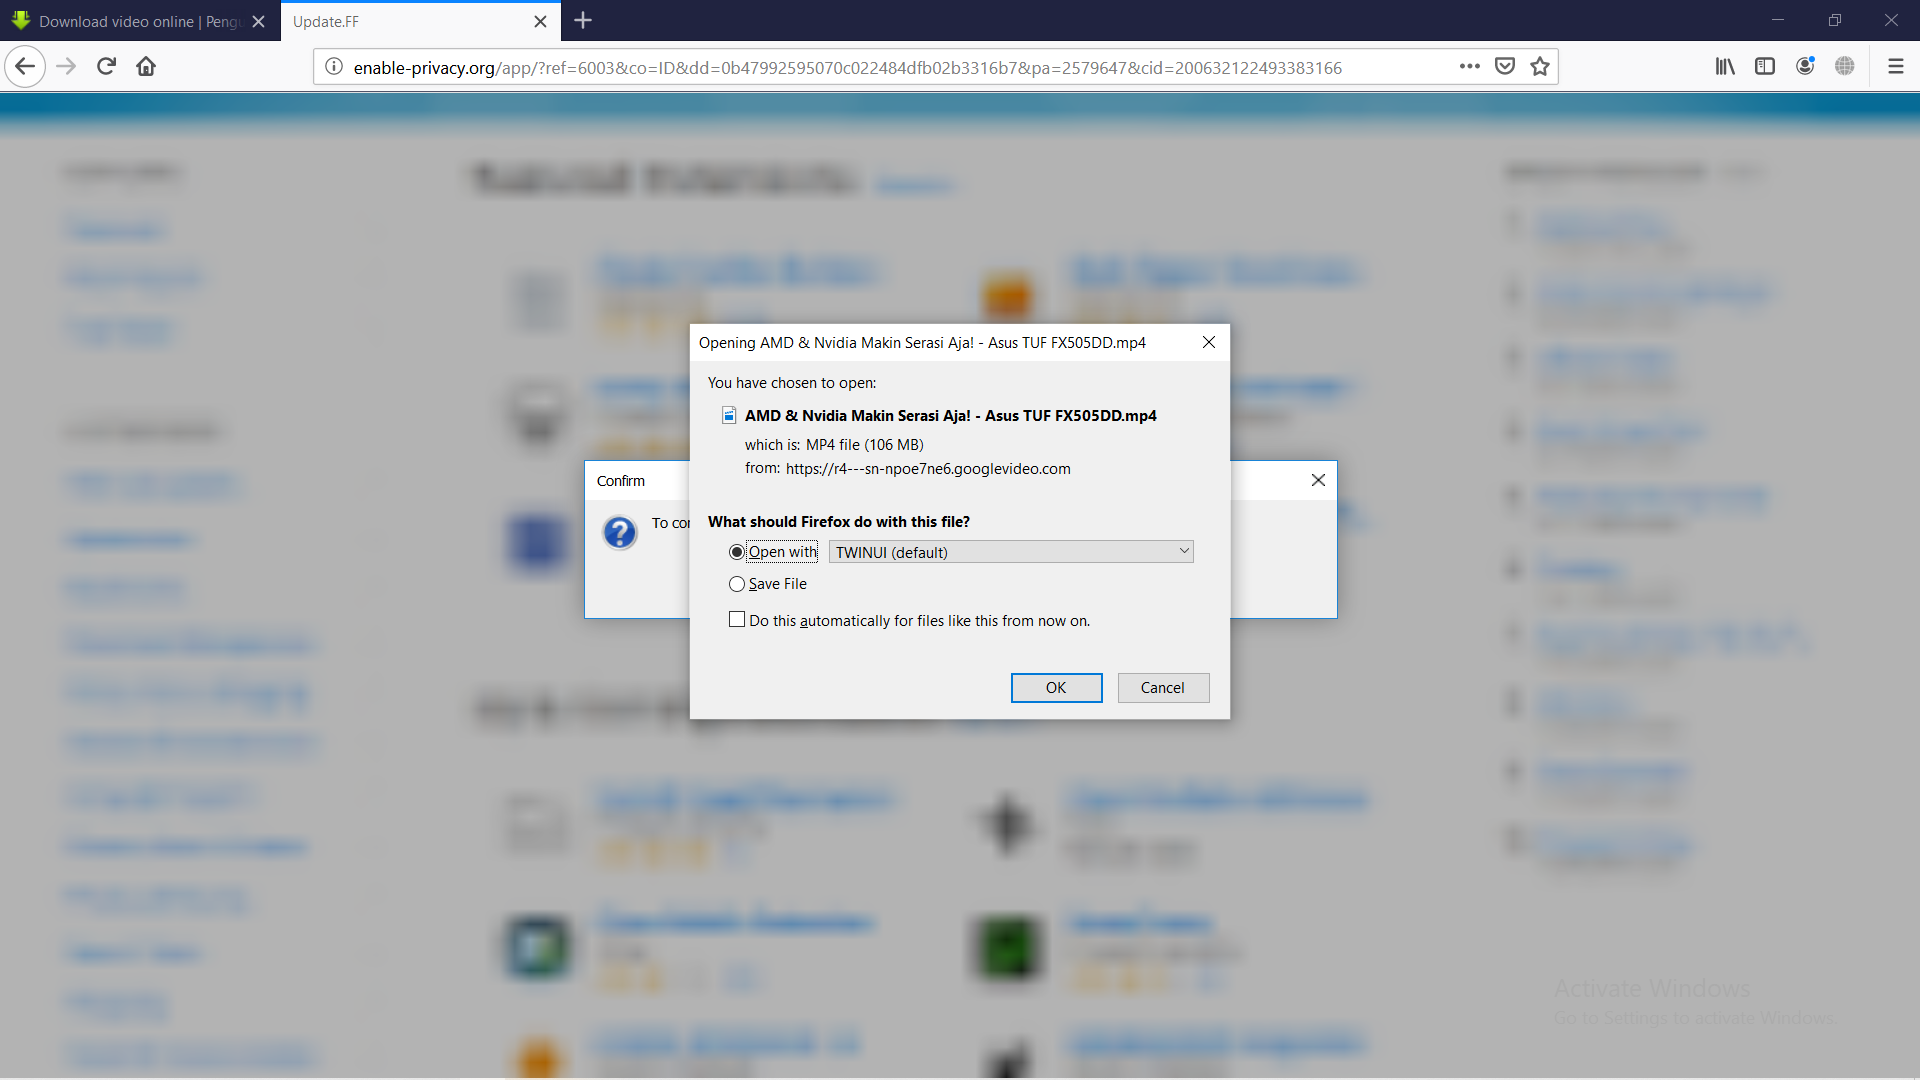
\includegraphics[scale=0.4]{figure/Antarmuka/9.png}
    \caption{ Proses saat video bisa di download}
    \label{gambar 1}
\end{figure}